\documentclass{practice}

\title{3}
\date{\DTMdate{2024-09-25}}

\usetikzlibrary{positioning,calc}

\begin{document}
\maketitle

\begin{task}{Every day I'm shufflin'}
  Consider the S-box defined by:
  \begin{table}[h!]
    \centering
    \begin{tabular}{|c|c|c|c|c|}
      \hline
      $S$ & \texttt{00} & \texttt{01} & \texttt{10} & \texttt{11}\\\hline
      \texttt{00} & \texttt{0000} & \texttt{1101} & \texttt{0110} & \texttt{1111} \\
      \texttt{01} & \texttt{1010} & \texttt{1011} & \texttt{0010} & \texttt{1010} \\
      \texttt{10} & \texttt{0100} & \texttt{1011} & \texttt{1110} & \texttt{1101} \\
      \texttt{11} & \texttt{1100} & \texttt{0101} & \texttt{0010} & \texttt{1001}\\\hline
    \end{tabular}
    \vspace*{-0.7em}
  \end{table}

  where the column is determined by the two least significant bits of a \emph{nibble} and the row is determined by the two most significant bits of a nibble.

  Given the round keys
  \[
    k_0 = \texttt{0x912C},\qquad
    k_1 = \texttt{0x35D3},\qquad
    k_2 = \texttt{0x229F},\qquad
    k_3 = \texttt{0x717A},
  \]
  encrypt the message \texttt{0x5350} using the SP-network described below:
 
  \begin{figure}[h!]
    \centering
    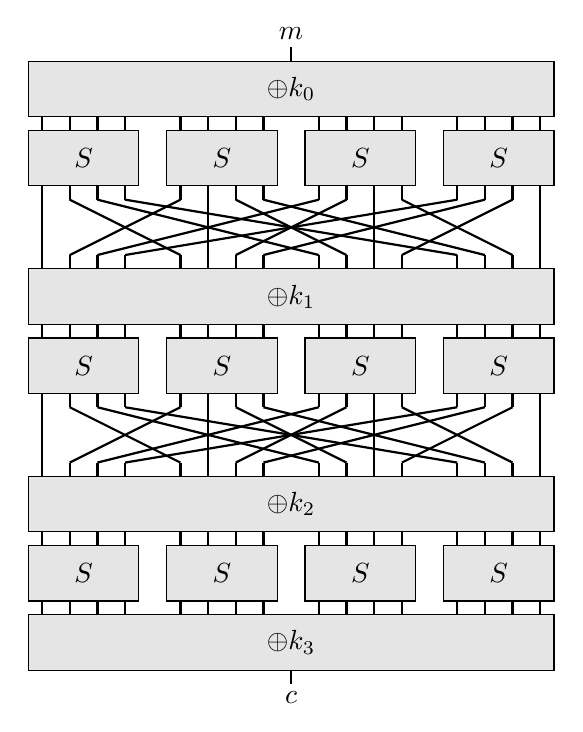
\begin{tikzpicture}[every node/.style={inner sep=0,outer sep=0}]
  \foreach \x in {1,...,4} {
    \node (s-1-\x) at ($\x*(5em,0)$) [
      minimum width=4em,
      minimum height=2em,
      fill=gray!20,draw] {$S$};

    \node (b1-1-tb-\x) at ($(s-1-\x.north)-(1.5em,0)$) {};
    \node (b2-1-tb-\x) at ($(s-1-\x.north)-(0.5em,0)$) {};
    \node (b3-1-tb-\x) at ($(s-1-\x.north)+(0.5em,0)$) {};
    \node (b4-1-tb-\x) at ($(s-1-\x.north)+(1.5em,0)$) {};

    \node (b1-1-tt-\x) [above of=b1-1-tb-\x, node distance=0.5em] {};
    \node (b2-1-tt-\x) [above of=b2-1-tb-\x, node distance=0.5em] {};
    \node (b3-1-tt-\x) [above of=b3-1-tb-\x, node distance=0.5em] {};
    \node (b4-1-tt-\x) [above of=b4-1-tb-\x, node distance=0.5em] {};

    \node (b1-1-bt-\x) at ($(s-1-\x.south)-(1.5em,0)$) {};
    \node (b2-1-bt-\x) at ($(s-1-\x.south)-(0.5em,0)$) {};
    \node (b3-1-bt-\x) at ($(s-1-\x.south)+(0.5em,0)$) {};
    \node (b4-1-bt-\x) at ($(s-1-\x.south)+(1.5em,0)$) {};

    \node (b1-1-bb-\x) [below of=b1-1-bt-\x, node distance=0.5em] {};
    \node (b2-1-bb-\x) [below of=b2-1-bt-\x, node distance=0.5em] {};
    \node (b3-1-bb-\x) [below of=b3-1-bt-\x, node distance=0.5em] {};
    \node (b4-1-bb-\x) [below of=b4-1-bt-\x, node distance=0.5em] {};

    \draw[thick] ($(b1-1-tb-\x)$) -- ($(b1-1-tt-\x)$);
    \draw[thick] ($(b2-1-tb-\x)$) -- ($(b2-1-tt-\x)$);
    \draw[thick] ($(b3-1-tb-\x)$) -- ($(b3-1-tt-\x)$);
    \draw[thick] ($(b4-1-tb-\x)$) -- ($(b4-1-tt-\x)$);

    \draw[thick] ($(b1-1-bt-\x)$) -- ($(b1-1-bb-\x)$);
    \draw[thick] ($(b2-1-bt-\x)$) -- ($(b2-1-bb-\x)$);
    \draw[thick] ($(b3-1-bt-\x)$) -- ($(b3-1-bb-\x)$);
    \draw[thick] ($(b4-1-bt-\x)$) -- ($(b4-1-bb-\x)$);

    \node (b1-k1-tt-\x) [below of=b1-1-bb-\x, node distance=2em] {};
    \node (b2-k1-tt-\x) [below of=b2-1-bb-\x, node distance=2em] {};
    \node (b3-k1-tt-\x) [below of=b3-1-bb-\x, node distance=2em] {};
    \node (b4-k1-tt-\x) [below of=b4-1-bb-\x, node distance=2em] {};

    \node (b1-k1-tb-\x) [below of=b1-k1-tt-\x, node distance=0.5em] {};
    \node (b2-k1-tb-\x) [below of=b2-k1-tt-\x, node distance=0.5em] {};
    \node (b3-k1-tb-\x) [below of=b3-k1-tt-\x, node distance=0.5em] {};
    \node (b4-k1-tb-\x) [below of=b4-k1-tt-\x, node distance=0.5em] {};

    \draw[thick] ($(b1-k1-tt-\x)$) -- ($(b1-k1-tb-\x)$);
    \draw[thick] ($(b2-k1-tt-\x)$) -- ($(b2-k1-tb-\x)$);
    \draw[thick] ($(b3-k1-tt-\x)$) -- ($(b3-k1-tb-\x)$);
    \draw[thick] ($(b4-k1-tt-\x)$) -- ($(b4-k1-tb-\x)$);
  }

  \foreach \x in {1,...,4} {
    \node (s-2-\x) at ($\x*(5em,0)-(0, 7.5em)$) [
      minimum width=4em,
      minimum height=2em,
      fill=gray!20,draw] {$S$};

    \node (b1-2-tb-\x) at ($(s-2-\x.north)-(1.5em,0)$) {};
    \node (b2-2-tb-\x) at ($(s-2-\x.north)-(0.5em,0)$) {};
    \node (b3-2-tb-\x) at ($(s-2-\x.north)+(0.5em,0)$) {};
    \node (b4-2-tb-\x) at ($(s-2-\x.north)+(1.5em,0)$) {};

    \node (b1-2-tt-\x) [above of=b1-2-tb-\x, node distance=0.5em] {};
    \node (b2-2-tt-\x) [above of=b2-2-tb-\x, node distance=0.5em] {};
    \node (b3-2-tt-\x) [above of=b3-2-tb-\x, node distance=0.5em] {};
    \node (b4-2-tt-\x) [above of=b4-2-tb-\x, node distance=0.5em] {};

    \node (b1-2-bt-\x) at ($(s-2-\x.south)-(1.5em,0)$) {};
    \node (b2-2-bt-\x) at ($(s-2-\x.south)-(0.5em,0)$) {};
    \node (b3-2-bt-\x) at ($(s-2-\x.south)+(0.5em,0)$) {};
    \node (b4-2-bt-\x) at ($(s-2-\x.south)+(1.5em,0)$) {};

    \node (b1-2-bb-\x) [below of=b1-2-bt-\x, node distance=0.5em] {};
    \node (b2-2-bb-\x) [below of=b2-2-bt-\x, node distance=0.5em] {};
    \node (b3-2-bb-\x) [below of=b3-2-bt-\x, node distance=0.5em] {};
    \node (b4-2-bb-\x) [below of=b4-2-bt-\x, node distance=0.5em] {};

    \draw[thick] ($(b1-2-tb-\x)$) -- ($(b1-2-tt-\x)$);
    \draw[thick] ($(b2-2-tb-\x)$) -- ($(b2-2-tt-\x)$);
    \draw[thick] ($(b3-2-tb-\x)$) -- ($(b3-2-tt-\x)$);
    \draw[thick] ($(b4-2-tb-\x)$) -- ($(b4-2-tt-\x)$);

    \draw[thick] ($(b1-2-bt-\x)$) -- ($(b1-2-bb-\x)$);
    \draw[thick] ($(b2-2-bt-\x)$) -- ($(b2-2-bb-\x)$);
    \draw[thick] ($(b3-2-bt-\x)$) -- ($(b3-2-bb-\x)$);
    \draw[thick] ($(b4-2-bt-\x)$) -- ($(b4-2-bb-\x)$);

    \node (b1-k2-tt-\x) [below of=b1-2-bb-\x, node distance=2em] {};
    \node (b2-k2-tt-\x) [below of=b2-2-bb-\x, node distance=2em] {};
    \node (b3-k2-tt-\x) [below of=b3-2-bb-\x, node distance=2em] {};
    \node (b4-k2-tt-\x) [below of=b4-2-bb-\x, node distance=2em] {};

    \node (b1-k2-tb-\x) [below of=b1-k2-tt-\x, node distance=0.5em] {};
    \node (b2-k2-tb-\x) [below of=b2-k2-tt-\x, node distance=0.5em] {};
    \node (b3-k2-tb-\x) [below of=b3-k2-tt-\x, node distance=0.5em] {};
    \node (b4-k2-tb-\x) [below of=b4-k2-tt-\x, node distance=0.5em] {};

    \draw[thick] ($(b1-k2-tt-\x)$) -- ($(b1-k2-tb-\x)$);
    \draw[thick] ($(b2-k2-tt-\x)$) -- ($(b2-k2-tb-\x)$);
    \draw[thick] ($(b3-k2-tt-\x)$) -- ($(b3-k2-tb-\x)$);
    \draw[thick] ($(b4-k2-tt-\x)$) -- ($(b4-k2-tb-\x)$);
  }

  \foreach \x in {1,...,4} {
    \node (s-3-\x) at ($\x*(5em,0)-(0, 15em)$) [
      minimum width=4em,
      minimum height=2em,
      fill=gray!20,draw] {$S$};

    \node (b1-3-tb-\x) at ($(s-3-\x.north)-(1.5em,0)$) {};
    \node (b2-3-tb-\x) at ($(s-3-\x.north)-(0.5em,0)$) {};
    \node (b3-3-tb-\x) at ($(s-3-\x.north)+(0.5em,0)$) {};
    \node (b4-3-tb-\x) at ($(s-3-\x.north)+(1.5em,0)$) {};

    \node (b1-3-tt-\x) [above of=b1-3-tb-\x, node distance=0.5em] {};
    \node (b2-3-tt-\x) [above of=b2-3-tb-\x, node distance=0.5em] {};
    \node (b3-3-tt-\x) [above of=b3-3-tb-\x, node distance=0.5em] {};
    \node (b4-3-tt-\x) [above of=b4-3-tb-\x, node distance=0.5em] {};

    \node (b1-3-bt-\x) at ($(s-3-\x.south)-(1.5em,0)$) {};
    \node (b2-3-bt-\x) at ($(s-3-\x.south)-(0.5em,0)$) {};
    \node (b3-3-bt-\x) at ($(s-3-\x.south)+(0.5em,0)$) {};
    \node (b4-3-bt-\x) at ($(s-3-\x.south)+(1.5em,0)$) {};

    \node (b1-3-bb-\x) [below of=b1-3-bt-\x, node distance=0.5em] {};
    \node (b2-3-bb-\x) [below of=b2-3-bt-\x, node distance=0.5em] {};
    \node (b3-3-bb-\x) [below of=b3-3-bt-\x, node distance=0.5em] {};
    \node (b4-3-bb-\x) [below of=b4-3-bt-\x, node distance=0.5em] {};

    \draw[thick] ($(b1-3-tb-\x)$) -- ($(b1-3-tt-\x)$);
    \draw[thick] ($(b2-3-tb-\x)$) -- ($(b2-3-tt-\x)$);
    \draw[thick] ($(b3-3-tb-\x)$) -- ($(b3-3-tt-\x)$);
    \draw[thick] ($(b4-3-tb-\x)$) -- ($(b4-3-tt-\x)$);

    \draw[thick] ($(b1-3-bt-\x)$) -- ($(b1-3-bb-\x)$);
    \draw[thick] ($(b2-3-bt-\x)$) -- ($(b2-3-bb-\x)$);
    \draw[thick] ($(b3-3-bt-\x)$) -- ($(b3-3-bb-\x)$);
    \draw[thick] ($(b4-3-bt-\x)$) -- ($(b4-3-bb-\x)$);
  }

  % P-boxes

  \foreach \i in {1,2} {
    \draw[thick] ($(b1-\i-bb-1)$) -- ($(b1-k\i-tt-1)$);
    \draw[thick] ($(b4-\i-bb-4)$) -- ($(b4-k\i-tt-4)$);

    \draw[thick] ($(b2-\i-bb-1)$) -- ($(b1-k\i-tt-2)$);
    \draw[thick] ($(b3-\i-bb-4)$) -- ($(b4-k\i-tt-3)$);

    \draw[thick] ($(b3-\i-bb-1)$) -- ($(b1-k\i-tt-3)$);
    \draw[thick] ($(b2-\i-bb-4)$) -- ($(b4-k\i-tt-2)$);

    \draw[thick] ($(b4-\i-bb-1)$) -- ($(b1-k\i-tt-4)$);
    \draw[thick] ($(b1-\i-bb-4)$) -- ($(b4-k\i-tt-1)$);

    \draw[thick] ($(b1-\i-bb-2)$) -- ($(b2-k\i-tt-1)$);
    \draw[thick] ($(b4-\i-bb-3)$) -- ($(b3-k\i-tt-4)$);

    \draw[thick] ($(b2-\i-bb-2)$) -- ($(b2-k\i-tt-2)$);
    \draw[thick] ($(b3-\i-bb-3)$) -- ($(b3-k\i-tt-3)$);

    \draw[thick] ($(b2-\i-bb-2)$) -- ($(b2-k\i-tt-2)$);
    \draw[thick] ($(b3-\i-bb-3)$) -- ($(b3-k\i-tt-3)$);

    \draw[thick] ($(b3-\i-bb-2)$) -- ($(b2-k\i-tt-3)$);
    \draw[thick] ($(b2-\i-bb-3)$) -- ($(b3-k\i-tt-2)$);

    \draw[thick] ($(b4-\i-bb-2)$) -- ($(b2-k\i-tt-4)$);
    \draw[thick] ($(b1-\i-bb-3)$) -- ($(b3-k\i-tt-1)$);
  }

  % XOR boxes

  \foreach \i in {1,2} {
    \node (m{\i}t) at ($(b1-k\i-tb-1)!0.5!(b4-k\i-tb-4)$) {};
    \node (m{\i}m) [below of=m{\i}t, node distance=1em] {};
    \node[rectangle,draw,fill=gray!20,
      minimum height=2em,
      minimum width=19em] (r\i) at (m{\i}m) {$\oplus k_\i$};
  }

  \node (m0t) at ($(b1-1-tt-1)!0.5!(b4-1-tt-4)$) {};
  \node (m0m) [above of=m0t, node distance=1em] {};
  \node[rectangle,draw,fill=gray!20,
    minimum height=2em,
    minimum width=19em] (r0) at (m0m) {$\oplus k_0$};

  \node (m3t) at ($(b1-3-bb-1)!0.5!(b4-3-bb-4)$) {};
  \node (m3m) [below of=m3t, node distance=1em] {};
  \node[rectangle,draw,fill=gray!20,
    minimum height=2em,
    minimum width=19em] (r3) at (m3m) {$\oplus k_3$};

  % Input

  \node (in-b) at (r0.north) {};
  \node (in-t) [above of=in-b, node distance=0.5em] {};
  \draw[thick] ($(in-t)$) -- ($(in-b)$);
  \node (m) [above of=in-t, node distance=0.5em] {$m$};

  % Output

  \node (out-t) at (r3.south) {};
  \node (out-b) [below of=out-t, node distance=0.5em] {};
  \draw[thick] ($(out-t)$) -- ($(out-b)$);
  \node (ct) [below of=out-b, node distance=0.5em] {$c$};

\end{tikzpicture}
  \end{figure}
\end{task}

\newpage

\begin{task}{Down at the first round}
  Draw two rounds of the Feistel construction.
  Why is a single round of the construction not a pseudo-random permutation?
\end{task}

\begin{task}{DESperation}
  The DES expansion function is given by
  \begin{table}[h!]
    \centering
    \begin{tabular}{|c|c|c|c|c|c|}
      \hline
      32 &  1 &  2 &  3 &  4 &  5\\\hline
       4 &  5 &  6 &  7 &  8 &  9\\\hline
       8 &  9 & 10 & 11 & 12 & 13\\\hline
      12 & 13 & 14 & 15 & 16 & 17\\\hline
      16 & 17 & 18 & 19 & 20 & 21\\\hline
      20 & 21 & 22 & 23 & 24 & 25\\\hline
      24 & 25 & 26 & 27 & 28 & 29\\\hline
      28 & 29 & 30 & 31 & 32 &  1\\\hline
    \end{tabular}
    \vspace*{-0.7em}
  \end{table}

  Given the plaintext \texttt{0x45444553}, find the expanded plaintext.

\end{task}

\begin{task}{PRF? Is that you?}
  Let $F: \{0,1\}^\lambda \to \{0,1\}^\lambda$ be a secure PRF that we want to use to construct a PRF with longer input length.
  Below are some approaches\footnotemark{} that \emph{don't} work.
  For each one, describe a successful distinguisher.
  \footnotetext{Exercise 6.8 from the book \enquote{The Joy of Cryptography.}}%

  \begin{enumerate}
    \item $F'_k(x \vert\vert x') = F_k(x) \vert\vert F_k(x')$, where $x$ and $x'$ are each $\lambda$ bits long.
    \item $F'_k(x \vert\vert x') = F_k(x) \oplus F_k(x')$, where $x$ and $x'$ are each $\lambda$ bits long.
    \item $F'_k(x \vert\vert x') = F_k(x) \oplus F_k(x \oplus x')$, where $x$ and $x'$ are each $\lambda$ bits long.
    \item $F'_k(x \vert\vert x')= F_k(0\vert\vert x) \oplus F_k(1\vert\vert x')$, where $x$ and $x'$ are each $\lambda-1$ bits long.
  \end{enumerate}
\end{task}

\begin{task}{PRF from PRG}
  Let there be a secure PRG $G : \{0, 1\}^\lambda \to \{0, 1\}^{2\lambda}$.
  Show that the PRF $F_k(x) = G(k) \oplus x$ is not a secure PRF.
\end{task}

\newpage

\begin{task}{PRG from PRG}
  Let there be a secure PRG $G : \{0,1\}^\lambda \to \{0,1\}^{2\lambda}$.
  Let $s$ be a seed, and $G(s) = x\vert\vert y$.
  Show that the PRG $H(s)=G(s)\vert\vert G(y)$ is not a secure PRG.
\end{task}

\begin{task}{To Feistel or not to Feistel\dots}
  Think about S-boxes and their role in encryption.
  Why do we need the Feistel construction at all if SP-networks exist?
\end{task}
\end{document}
